\documentclass{scrartcl}
%\documentclass{article}
\usepackage[ngerman]{babel}
\usepackage[utf8]{inputenc}
\usepackage{courier}
\usepackage{amsmath}
\usepackage{graphicx}
\usepackage{tabularx}
\usepackage{hyperref}
\usepackage{amssymb}
\usepackage{verbatim}
\newcommand{\name}[1]{\textbf{\texttt{#1}}}
\newcommand{\add}{
    \renewcommand{\labelitemi}{+}
    \item
    \renewcommand{\labelitemi}{•}
}
\newcommand{\remove}{
    \renewcommand{\labelitemi}{-}
    \item
    \renewcommand{\labelitemi}{•}
}
\newcommand{\change}{
    \renewcommand{\labelitemi}{!}
    \item
    \renewcommand{\labelitemi}{•}
}
\begin{document}
\title{
    \hspace{-0.5cm} 
\includegraphics[height=5cm]{../../pflichtenheft/resources/logo.png} \\[1cm]
    \Huge{YUV.KA - Implementierungsheft} \\ \large{Praxis der Softwareentwicklung 2011/2012}
}
\author{Max Wagner $\cdot$ Patrick Gemander $\cdot$ Sebastian Ullrich $\cdot$ Michael Vollmer \\ Robert Hangu $\cdot$ Daniel Lebert}
\maketitle

\newpage
\mbox{}
\newpage
\mbox{}

\addcontentsline{toc}{section}{Inhaltsverzeichnis}
\tableofcontents
\clearpage

\section{Aktuelles Klassendiagramm}
\subsection{VideoModel}
\begin{figure}[h!]
\begin{center}
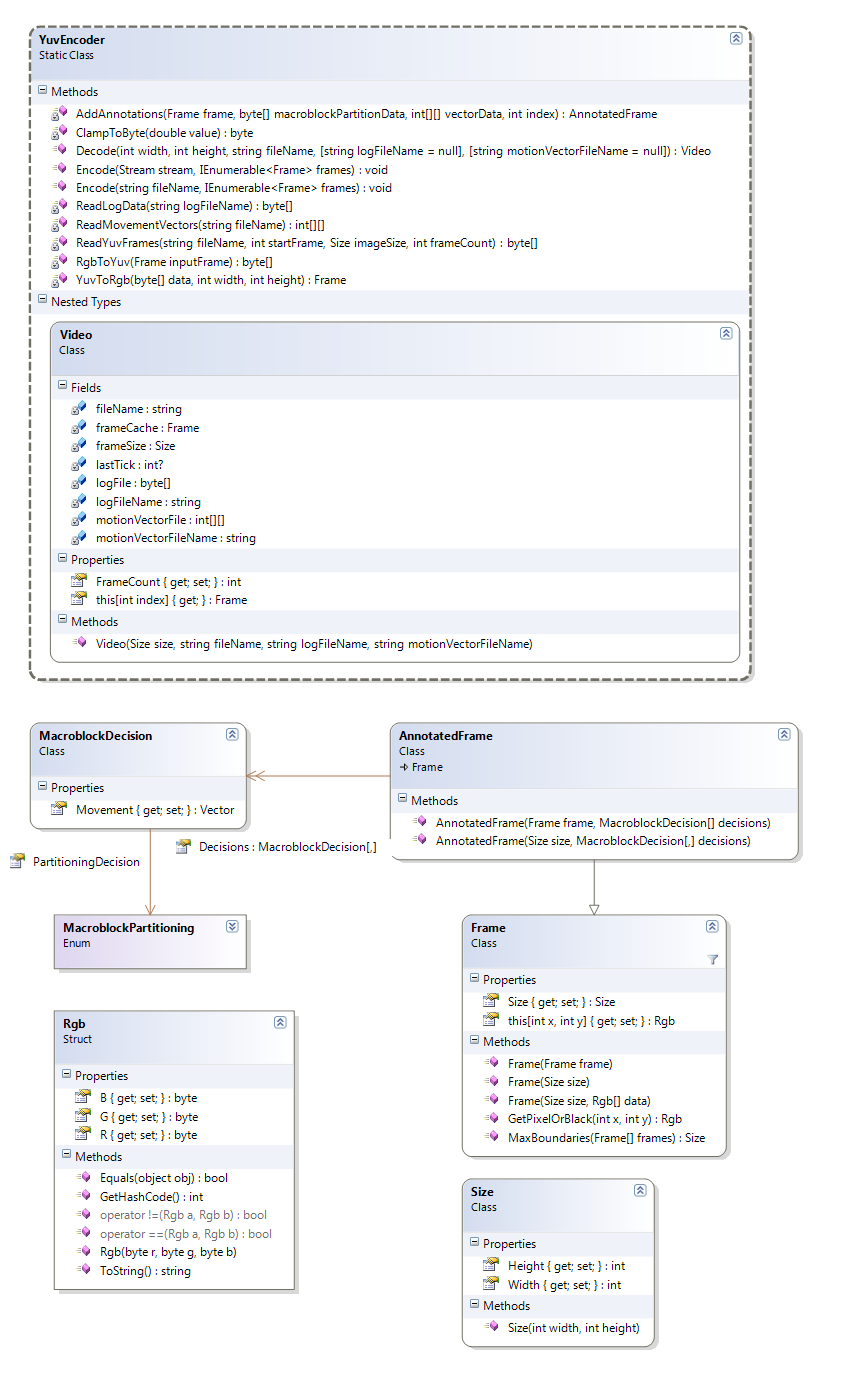
\includegraphics[height=0.8\textheight]{classdiagram/videomodel.png}
\end{center}
\end{figure}
\newpage

\subsection{Model}
\begin{figure}[h!]
\begin{center}
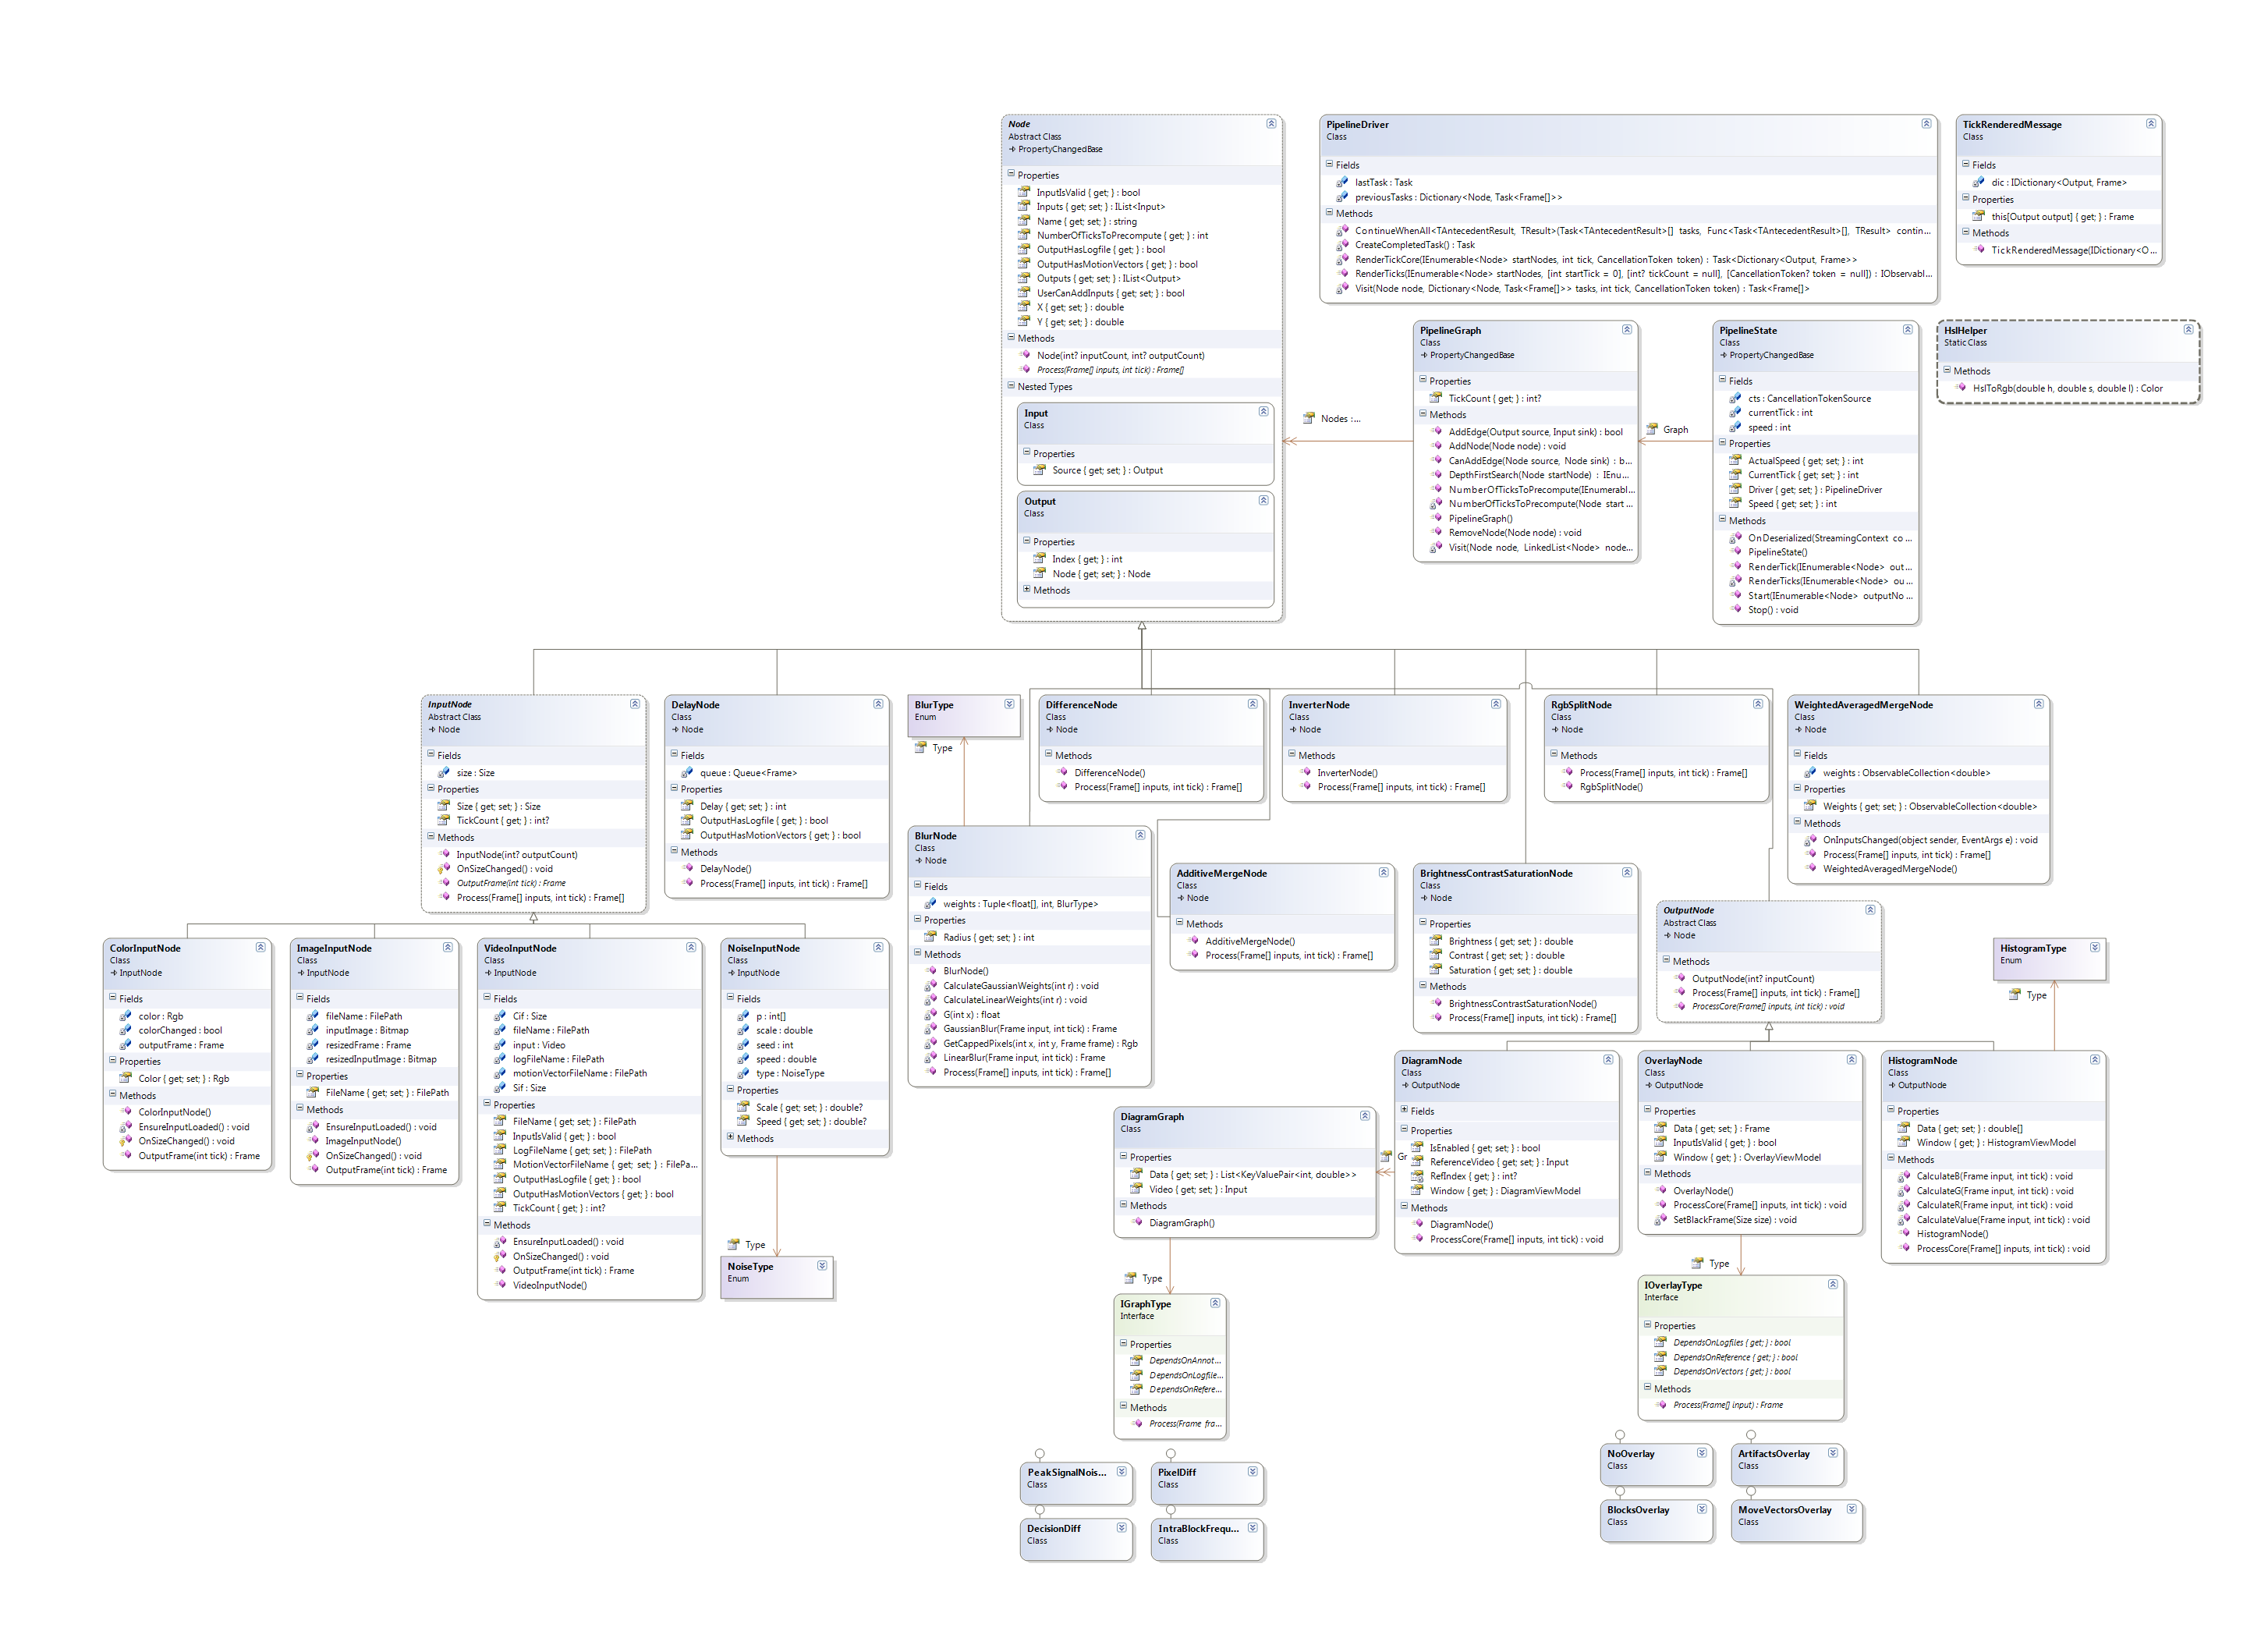
\includegraphics[width=0.9\textheight,angle=90]{classdiagram/model.png}
\end{center}
\end{figure}
\newpage

\subsection{ViewModel}
\begin{figure}[h!]
\begin{center}
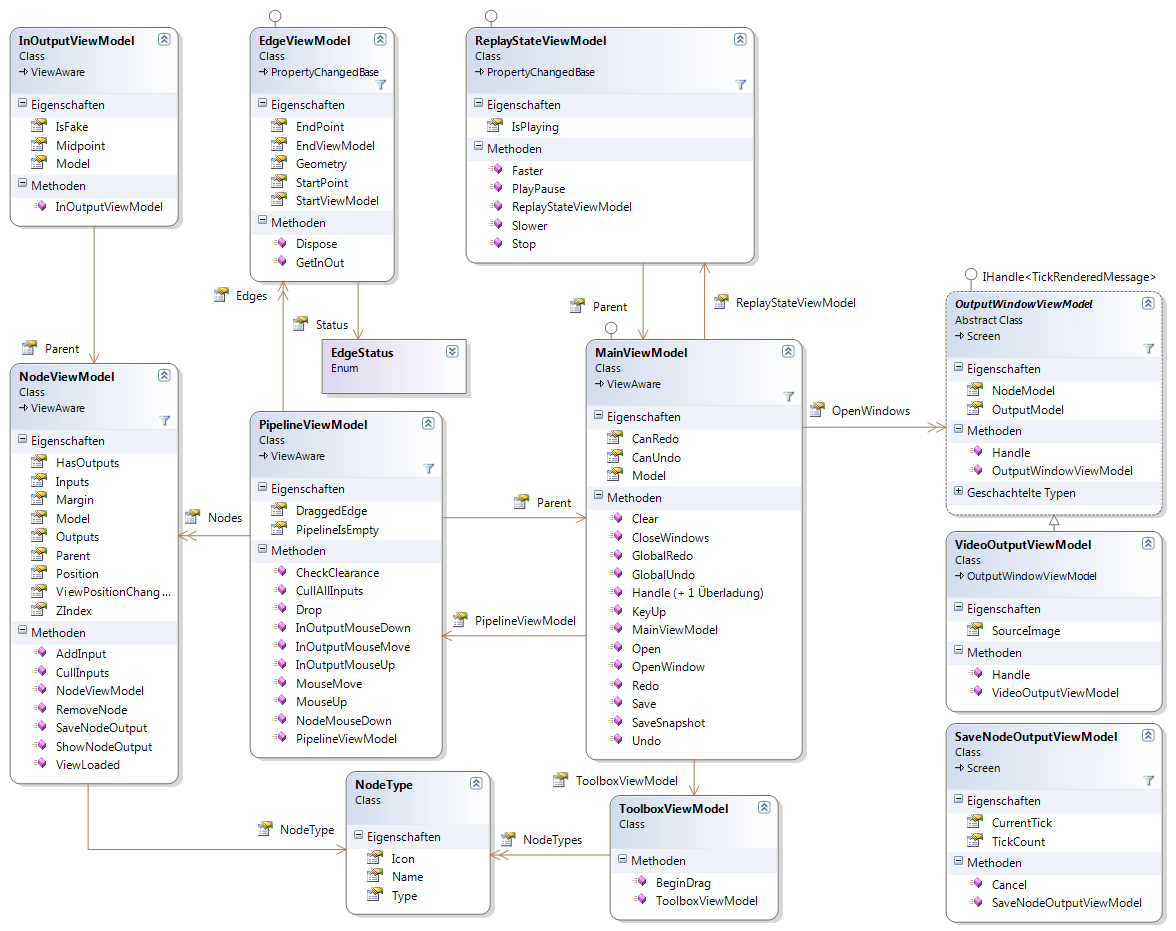
\includegraphics[width=0.8\textheight,angle=90]{classdiagram/viewmodel.png}
\end{center}
\end{figure}
\newpage

\subsection{PropertyViewModel}
\begin{figure}[h!]
\begin{center}
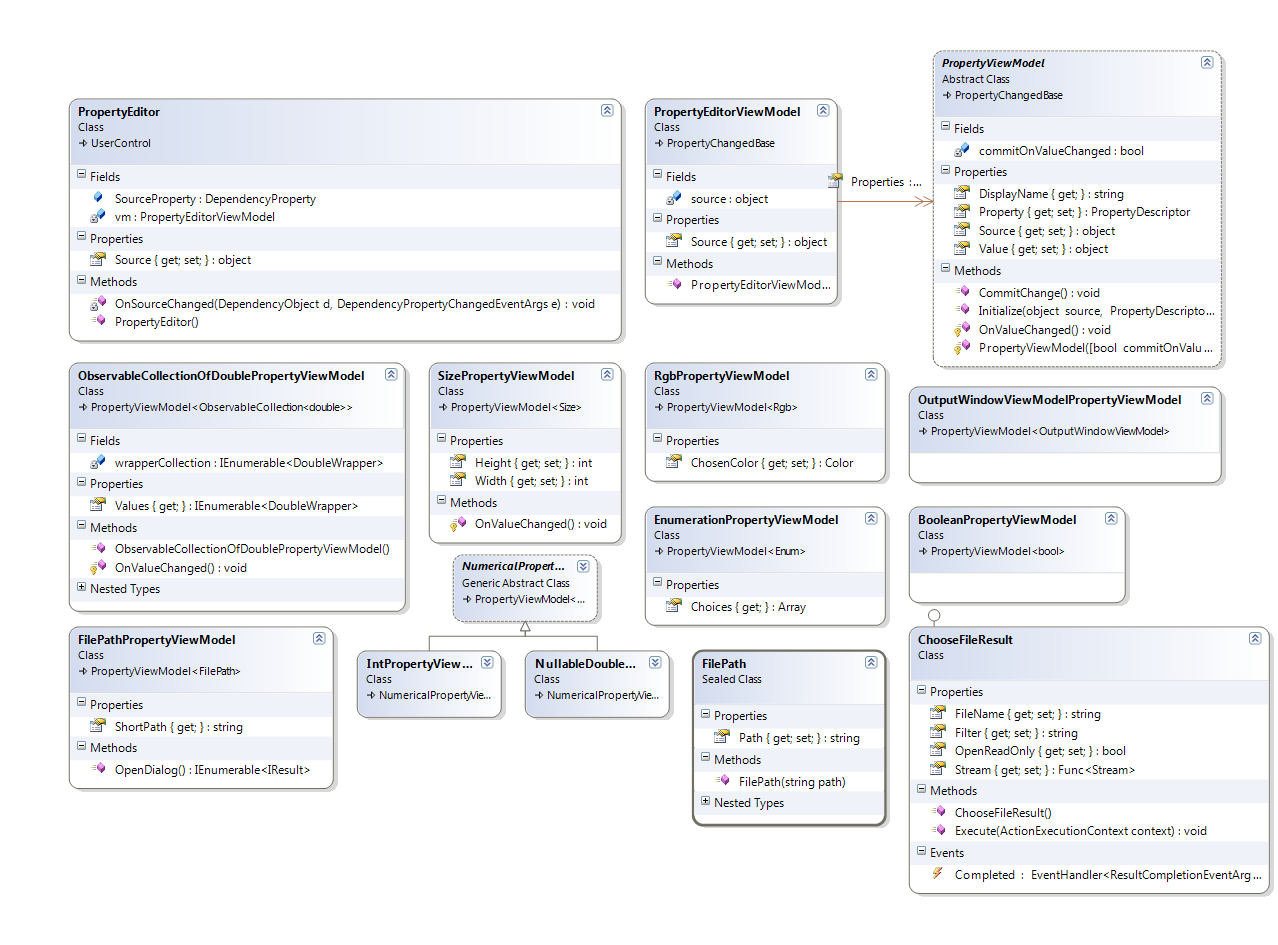
\includegraphics[height=0.7\textheight]{classdiagram/propertyeditorvm.png}
\end{center}
\end{figure}
\newpage
\clearpage

\section{Architekturänderungen}
\subsection{\name{YuvKA.VideoModel}}

\paragraph{\name{Frame}}
\begin{itemize}
	\add \verb!public GetPixelOrBlack(int x, int y)! \\
	Neue öffentliche Methode, die es erleichtern soll, auf die Farbwerte innerhalb eines Frames zuzugreifen, ohne beachten zu müssen, ob die gegebenen Koordinaten tatsächlich innerhalb des \name{Frame} liegen. Falls ja, so wird der entsprechende Pixel an Stelle (x, y) als \name{Rgb}-Objekt zurückgegeben. Falls nicht, so wird ein schwarzer Farbwert für den Pixel zurückgegeben.
	\add \verb!public MaxBoundaries(Frame[] frames)! \\
	Neue öffentliche Methode, welche aus einem Array von Frames jeweils das Maximum der Breite und der Höhe findet und ein \name{Size}-Objekt zurückgibt mit \name{height}- bzw. \name{width}-Wert, welcher alle gegebenen Frames umfasst.
\end{itemize}

\paragraph{\name{MacroblockDecision}}
\begin{itemize}
	\change \verb!public Vector Movement { get; set; }! \\
	Die \name{Movement}-property wurde schreibbar gemacht, da eine korrekte Initialisierung sonst nicht möglich wäre.
	\change \verb!public MacroblockPartitioning? Partitiondecision { get; set; }! \\
	Die \name{Partitiondecision}-property wurde schreibbar gemacht, da eine korrekte Initialisierung sonst nicht möglich wäre.
\end{itemize}

\paragraph{\name{Rgb}}
\begin{itemize}
	\change \verb!public byte R { get; private set; }! \\
	Der setter der R-Property wurde auf private gesetzt.
	\change \verb!public byte G { get; private set; }! \\
	Der setter der G-Property wurde auf private gesetzt.
	\change \verb!public byte B { get; private set; }! \\
	Der setter der B-Property wurde auf private gesetzt.
\end{itemize}

\paragraph{\name{YuvEncoder}}
\begin{itemize}
	\add \verb!public static Video Decode(int width, int height, string filename, string logFileName = null, string motionVectorFileName = null)! \\
	Neuer Parameter \verb!string motionVectorFileName = null!: Die an ein Video gebundenen Bewegungsvektoren sollen schon beim Lesen eines Videos vom Hintergrundspeicher gelesen werden, da \name{Video}-Obekte unveränderlich sind, und bei Neuwahl der entsprechenden Datei ein neues Video-Objekt erstellt werden muss.
	\add \verb!public static void Encode(Stream stream, IEnumerable<Frame> frames)! \\
	Neue öffentliche statische Methode Encode, welche als Parameter einen Stream entgegennimmt. Dies ermöglicht es, zu Testzwecken auch in einen \name{MemoryStream} zu schreiben, was den Hintergrundspeicher nicht belastet und in der Regel schneller ist.
\end{itemize}

\paragraph{\name{YuvEncoder.Video}}
\begin{itemize}
	\remove \verb!public void Dispose()! \\
	Da keine Streams länger als unbedingt nötig offen gehalten werden, ist die zuvor von der \name{Video}-Klasse implementierte Schnittstelle \name{IDisposable} hier nicht mehr benötigt. Dadurch entfällt diese Methode.
\end{itemize}


\subsection{\name{YuvKA.Pipeline}}

\paragraph{\name{InputNode}}
\begin{itemize}
	\change \verb!public int? TickCount! \\
	Die Property \verb!TickCount! ist nun nullable. Der Wert null steht hierbei für die Möglichkeit (theoretisch) unendlich viele Frames zu erzeugen.
\end{itemize}

\paragraph{\name{Node}}
\begin{itemize}
	\change \verb!public Node(int? inputCount, int? outputCount)! \\
	Die Parameter des Konstruktors sind jetzt nullable, um mit dem Wert null eine Variable Anzahl von Ein-/Ausgängen zu repräsentieren.
	\add \verb!public virtual bool InputIsValid { get; }! \\
	Diese Property wurde eingeführt, um repräsentieren zu können, ob alle Inputs des Knotens (indirekt) mit InputNodes verbunden sind und der Knoten somit seine Berechnung auch ausführen kann.
	\add \verb!public string Name { get; set; }! \\
	Repräsentiert den Namen des Knoten. Der Name eines Knoten ist eine möglichst kurze Beschreibung der Funktionsweise des Knotens. Im Idealfall ist diese Beschreibung nur ein Wort lang.
	\add \verb!public virtual int NumberOfFramesToPrecompute { get; }! \\
	Wurde eingeführt, da manche Knoten Daten aus vergangenen Ticks zur Berechnung des aktuellen Ticks brauchen. Damit diese Knoten auch nach dem Springen in der Pipeline das korrekte Ergebnis liefern, muss man eventuell Ticks vorberechnen. Diese Property repräsentiert, wie viele vergangene Frames der Knoten kennen muss, um seine Berechnung auszuführen.
	\add \verb!public virtual bool OutputHasLogfile { get; }! \\
	Wurde eingeführt, um repräsentieren zu können, ob die Ausgabe des Knotens Logfiles beinhaltet.
	\add \verb!public virtual bool OutputHasMovementVectors { get; }! \\
	Wurde eingeführt, um repräsentieren zu können, ob die Ausgabe Movement-Vektoren beinhaltet.
	\add \verb!public virtual bool UserCanAddInputs { get; }! \\
	Diese Property gibt an, ob der User in der Lage sein soll Inputs zu diesem Knoten hinzuzufügen.
	\remove \verb!public void Dispose()! \\
	Die Methode \verb!Dispose()! wurde entfernt, da keine Streams mehr offen gehalten werden.
\end{itemize}

\paragraph{\name{Node.Input}}
\begin{itemize}
	\remove \verb!public int Index { get; }! \\
	Wurde entfernt, da es nicht mehr gebraucht wurde und Node.Input keinen Zugriff auf seinen Knoten hat und daher seinen Index auch nicht berechnen kann.	
\end{itemize}

\paragraph{\name{PipelineDriver}}
\begin{itemize}
	\change Die Klasse ist nicht mehr als statisch deklariert. Diese Änderung ermöglicht, verschiedene Graphen parallel zu berechnen, indem jeweils ein Driver instanziert wird, die einzelnen Berechnungen aber weiterhin den Parallelitätszusicherungen genügen.
	\add \verb!public IObservable<IDictionary<Node.Output, Frame>> RenderTicks(IEnumerable<Node> startNodes, int startTick = 0, int? tickCount = null, CancellationToken? token = null)! \\
	Neuer Parameter \verb!int? tickCount = null!: Wie sich herausstellte, sollte die Berechnung der Pipeline nicht nur durch ein \name{CancellationToken} jederzeit abbrechbar sein, sondern auch von sich aus nach einer gegebenen Anzahl Ticks, nämlich bis zum Ende des gegebenen Eingabevideos, enden können. Existiert kein Eingabevideo, kann dem Parameter \name{null} zugewiesen werden (der Standardwert), um weiterhin bis zu einem manuellen Abbruch zu berechnen.
\end{itemize}

\paragraph{\name{PipelineGraph}}
\begin{itemize}
	\change \verb!public int? TickCount { get; }! \\
	Die Property ist nun ein nullable int, da der Wert Null verwendet wird, um eine unbegrenzte Videolänge zu signalisieren.
	\add \verb!public void AddNode(Node node)! \\
	Diese Erweiterung ermöglicht es beim Hinzufügen eines Knoten diesem einen eindeutigen Namen aus der Folge Defaultname, Defaultname 2, Defaultname 3, ... zuzuordnen. Dieser Name kann nun verwendet werden, um ihn im Knoten selbst und allen seinen zugehörigen Outputfenstern anzuzeigen. Hiermit steht dem Benutzer eine leiche erkennbare eindeutige Zuordnung zur Verfügung. Weiterhin sollten auf keine andere Weise Knoten zum Graphen hinzugefügt werden.
	\add \verb!public bool CanAddEdge(Node source, Node sink)! \\
	Die Abfrage, ob eine Kante legal ist, ohne sie auch hinzuzufügen, ermöglicht es, Kanten in der GUI schon vor dem Drop-Event als legal oder illegal zu markieren.
	\add \verb!public int NumberOfFramesToPrecompute(IEnumerable<Node> outputNodes)! \\
	Da es möglich sein soll in der Pipeline zu springen und es Knoten gibt, die den aktuellen Frame aus vergangenen Ticks berechnen, muss hierzu errechnet werden wie viele Ticks vorberechnet werden sollen.
	\add \verb!public void RemoveNode(Node node)! \\
	Es stellte sich heraus, dass beim Entfernen eines Knoten aus dem Graphen auch alle zugehörigen Kanten entfernt werden müssen. Diese neue Methode ermöglicht dies.
\end{itemize}

\paragraph{\name{PipelineState}}
\begin{itemize}
	\add \verb!public int ActualSpeed { get; }! \\
	Besonders zu Debugzwecken und zur Demonstration wurde diese Property hinzugefügt, um die tatsächlich gemessene Abarbeitungsgeschwindigkeit in der UI anzeigen zu können.
	\add \verb!public PipelineDriver Driver { get; }! \\
	Nachdem in der \name{PipelineDriver}-Klasse der \name{static}-Modifier entfernt wurde, musste mit dieser neuen Property der Pipeline eine Driver-Instanz zugeordnet werden.
\end{itemize}


\subsection{\name{YuvKA.Pipeline.Implementation}}

\paragraph{\name{AveragedMergeNode}}
\begin{itemize}
	\change Wurde zu WeightedAveragedMergeNode umbenannt, da es die Funktion des Knotens besser beschreibt.
\end{itemize}

\paragraph{\name{NoiseInputNode}}
\begin{itemize}
	\add \verb!public double? Scale { get; set; }! \\
	Diese neu eingeführte Option erlaubt es dem Benutzer den angezeigten Perlin Noise zu skalieren.
	\add \verb!public double? Speed { get; set; }! \\
	Diese neu eingeführte Option erlaubt es dem Benutzer die Geschwindigkeit des angezeigten Perlin Noise einzustellen.
\end{itemize}

Desweiteren wurden zwei neue Arten von Noise eingeführt, die Abwandlungen der schon existierenden sind (siehe \name{NoiseType}).

\paragraph{\name{NoiseType}}
\begin{itemize}
	\add \verb!ColoredCoherent! \\
	Erstellt farbigen Coherent Noise.
	\add \verb!ColoredPerlin! \\
	Erstellt farbigen Perlin Noise.
\end{itemize}

\paragraph{\name{DiagramGraph}}
\begin{itemize}
	\change \verb!public IList<KeyValuePair<int, double>> Data { get; set; }! \\
	Der Liste wurde jeweils der Tick des zugehörigen Analysedatums hinzugefügt.
\end{itemize}

\paragraph{\name{IGraphType}}
\begin{itemize}
	\add \verb!bool DependsOnAnnotatedReference { get; }! \\
	Ruft ab, ob der Diagrammtyp ein Referenzvideo mit Logfile benötigt.
	\add \verb!bool DependsOnLogfile { get; }! \\
	Ruft ab, ob der Diagrammtyp ein Logfile benötigt.
\end{itemize}

\paragraph{\name{HistogramNode}}
Die zur Berechnung des jeweiligen Histogrammtyps benötigten Methoden wurden als private Methoden ausgelagert.

\paragraph{\name{OverlayNode}}
\begin{itemize}
	\add \verb!public Frame Data { get; private set; }! \\
	Eine Schnittstelle durch die andere Klassen das Resultat der Überlagerung abgreifen können. Dies ist notwendig, da die \name{View} die \name{Process} Methode nicht selbst aufruft.
	\add \verb!public OverlayViewModel Window { get; }! \\
	Ruft das \name{OverlayViewModel}, welches zu diesem Knoten gehört, auf bzw. erstellt es. Dies ist notwendig, da die \name{View} wissen muss dass dieser Knotentyp, eine eigene Ausgabefensterart besitzt und sich dies mit einem entsprechenden \name{ProperyViewModel} ohne schwerwiegende Architektureingriffe sehr gut verwirklichen lässt.
\end{itemize}

\paragraph{\name{IOverlayType}}
\begin{itemize}
	\add \verb!bool DependsOnReference { get; }! \\
	Eine Wahrheitsvariable die wiedergibt, ob die Überlagerungsart auf eine Referenz angewiesen ist.
	\add \verb!bool DependsOnVectors { get; }! \\
	Eine Wahrheitsvariable die wiedergibt, ob die Überlagerungsart auf Bewegungsvektordaten angewiesen ist.
\end{itemize}

\paragraph{\name{+ NoOverlay}}~\\
Diese Klasse ist ein Überlagerungstyp der nichts überlagert und somit stets verfügbar ist, unabhängig von den zusätzlichen Daten neben der obligatorischen ursprünglichen \name{Frame}.

\subsection{\name{YuvKA.ViewModel}}

Wie erwartet hat sich im Viewmodel eine große Zahl an Änderungen ergeben, die zum Großteil aus dem Hinzufügen neuer Properties bestehen. Dies ist besonders der Tatsache geschuldet, dass das Viewmodel nicht wirklich Teil der grundlegenden Architektur sondern vielmehr Verknüpfungsschicht des Models und der View ist, wobei die Architektur letztgenannter Schicht, nämlich WPF, bereits gegeben war und wegen ihres unglaublichen Umfangs im Detail erst während der Implementierung Fall für Fall exakt erkundet werden konnte. Deshalb werden im Weiteren die Änderungen beschrieben, ohne einzeln auf die Gründe einzugehen, warum von der Entwurfsarchitektur abgewichen wurde.

\paragraph{\name{EdgeViewModel}}
\begin{itemize}
	\add \verb!public InOutputViewModel StartViewModel { get; set; }! \\
	     \verb!public InOutputViewModel EndViewModel { get; set; }! \\
	Legt Anfang bzw. Ende der Kante auf einen Ein-/Ausgang fest. Nach Setzen der Properties werden Start- bzw. Endpunkt der Kante automatisch entsprechend aktualisiert.
	\add \begin{verbatim}public EdgeStatus Status { get; set; }
	enum EdgeStatus { Indeterminate, Invalid, Valid }
	\end{verbatim}
	Gibt während des Ziehens einer Kante ihren Zustand an, der in der View durch die Linienfarben schwarz/rot/grün visualisiert wird.
	\add \verb!public void Dispose()! \\
	Entfernt alle Abonnements von Positionsänderungen der verbundenen Knoten, um Speicherlecks zu verhindern.
\end{itemize}

\paragraph{\name{+ InOutputViewModel}}~\\
\name{InOutputViewModel} ist eine gemeinsames View Model für Inputs und Outputs.
\begin{itemize}
	\add \verb!public bool IsFake { get; }! \\
	Fake-Eingänge sind solche ohne zugrundeliegendes Model. Sie werden für das dynamische Hinzufügen von Eingängen benötigt.
	\add \verb!public IObservable<Point> Midpoint { get; }! \\
	Gibt den gerade jeweils aktuellen Mittelpunkt des Ein-/Ausgangs zurück.
	\add \verb!public object Model { get; }! \\
	Der zugrundeliegende Input oder Output
	\add \verb!public NodeViewModel Parent { get; }! \\
	Das View Model des Knotens dieses Ein-/Ausgangs
\end{itemize}

\paragraph{\name{MainViewModel}}
\begin{itemize}
	\add \verb!public void CloseWindows(Node node)! \\
	Erzwingt das Schließen aller Ausgabefenster dieses Knotens
	\add \verb!public void Handle(OutputWindowViewModel.ClosedMessage message)! \\
	Reagiert auf das Schließen eines Fensters.
	\verb!public void Handle(ChangeCommittedMessage message)! \\
	Reagiert auf in sich abgeschlossene Wertänderungen von Knoten-Properties.
\end{itemize}

\paragraph{\name{NodeViewModel}}
\begin{itemize}
	\add \verb!public bool HasOutputs { get; }! \\
	Gibt an, ob der Knoten derzeit Ausgänge besitzt.
	\add \verb!public IEnumerable<InOutputViewModel> Inputs { get; }! \\
	\verb!public IEnumerable<InOutputViewModel> Outputs { get; }! \\
	Wrappen die Ein-/Ausgänge des Knotens in enstprechende View Models.
	\add \verb!public Thickness Margin { get; }! \\
	Gibt die durch \name{Position} angegebene Verschiebung View-verträglich zurück.
	\add \verb!public Point Position { get; set; }! \\
	Zusammenfassung des \name{X}- und \name{Y}-Wertes des Knotens
	\add \verb!public IObservable<Unit> ViewPositionChanged { get; }! \\
	Beobachtbare Sequenz von Events, in der jeder Eintrag für die Veränderung der tatsächlichen Position auf der View steht.
	\add \verb!public int ZIndex { get; set; }! \\
	Regelt die Zeichenabfolge von Knoten, damit der letztausgewählte Knoten nicht von anderen verdeckt ist.
	\add \verb!public void AddInput()! \\
	Fügt bei dynamisch um Eingänge erweiterbaren Knoten einen neuen Eingang hinzu.
	\add \verb!public void RemoveNode()! \\
	Entfernt diesen Knoten aus allen relevanten Listen und schließt alle Ausgabefenster des Knotens.
	\add \verb!public void ViewLoaded()! \\
	Eventhandler, um \name{ViewPositionChanged} initial zu triggern.
\end{itemize}

\paragraph{\name{NodeType}}
\begin{itemize}
	\add \verb!public string Name { get; set; }! \\
	Name des Knotens, der lesbarer ist als der reine Typname.
\end{itemize}

\paragraph{\name{PipelineViewModel}}
\begin{itemize}
	\add \verb!public EdgeViewModel DraggedEdge { get; }! \\
	Die gerade gezogene Kante, sonst null.
	\add \verb!public void CheckClearance(IDragEventInfo e)! \\
	Verhindert das Droppen eines Knoten, falls die Pipeline abgespielt wird.
	\change \verb!public void Drop(IDragEventInfo e)! \\
	Der Parametertyp wurde von WPFs \verb!DragEventArgs! auf das eigens kreierte Interface \name{IDragEventInfo} geändert, da ersterer Typ nicht mockbar ist.
	\add \begin{verbatim}
public void InOutputMouseDown(InOutputViewModel inOut)
public void InOutputMouseMove(InOutputViewModel inOut, RoutedEventArgs e)
public void InOutputMouseUp(InOutputViewModel inOut)
public void MouseMove(IMouseEventInfo e)
public void MouseUp()
public void NodeMouseDown(NodeViewModel inOut, IMouseEventInfo e)
	\end{verbatim}
	Eventhandler für Drag \& Drop
\end{itemize}

\paragraph{\name{ReplayStateViewModel}}
\begin{itemize}
	\change \verb!public bool IsPlaying { get; set; }! \\
	Der Setter wurde \verb!public! gemacht, damit das \name{MainViewModel} beim Laden einer Pipeline die Wiedergabe stoppen kann.
\end{itemize}

\paragraph{\name{VideoOutputViewModel}}
\begin{itemize}
	\add \verb!public WriteableBitmap SourceImage { get; }! \\
	Speichert das Bild, das als nächstes in das Ausgabefenster gezeichnet werden soll.
\end{itemize}


\subsection{\name{YuvKA.ViewModel.Implementation}}

\paragraph{\name{HistogramViewModel}}
\begin{itemize}
	\add \verb!public EnumerableDataSource<KeyValuePair<int, double>> Data { get; private set; }! \\
	Ruft die Analysedaten des Histogrammes ab oder setzt diese fest.
\end{itemize}

\paragraph{\name{DiagramViewModel}}
\begin{itemize}
	\add \verb!public ObservableCollection<LineGraphViewModel> LineGraphs { get; }! \\
	Ruft die Kurven im Diagramm ab, die den Graphen des Dieagrammknotens entsprechen. 
	\add \verb!public Tuple<string, Node.Input> Reference { get; set; }! \\
	Ruft das Referenzvideo des Diagrammknotens ab oder setzt diese fest.
	\add \verb!public ObservableCollection<Tuple<string, Node.Input>> Videos { get; }! \\
	Ruft die Eingabevideos des Diagrammknotens ab und fügt diesen einen Index hinzu.
	\add \verb!public public Tuple<string, Node.Input> ChosenVideo { get; set; }! \\
	Ruft das aktuell vom Benutzer zur Analyse ausgewählte Video ab oder setzt dieses fest.
	\add \verb!public ObservableCollection<GraphControl> GraphControls { get; set; }! \\
	Ruft die Grapheneinstellungen ab oder setzt diese fest.
	\add \verb!public List<Color> LineColors { get; set; }! \\
	Ruft die zur Zeichnung schon verwendeten Farben ab oder setzt diese fest.
	\add \verb!public List<System.Windows.Media.Color> TypeColors { get; }! \\
	Ruft die Basisfarben der einzelnen Graphtypen ab, von denen dann die einzelnen, zur Zeichnung verwendeten Farben abgeleitet werden.
	\change \verb!public IEnumerable<Tuple<string, IGraphType>> Types { get; set; }! \\
	Den Diagrammtypen wird nun ein Name hinzugefügt, damit dieser in der GUI angezeigt werden kann.
	\add \verb!public static bool IsInIntervall(double intervallCenter, double number, double intervallSize)! \\
	Entscheidet, ob eine Zahl in einem Intervall liegt.
	\add \verb!public void DeleteGraphControl(GraphControl graphControl)! \\
	Löscht eine gegebene Grapheneinstellung sowie deren Graph und dessen Kurve.
	\add \verb!public override void Handle(TickRenderedMessage message)! \\
	Aktualisiert jede Kurve mit den jewiligen Daten eines Frames, sobald dieser berechnet wurde.
	\change \verb!public void AddGraph(GraphControl graphControl)! \\
	Fügt eine Graphen und dessen Kurve hinzu, der aus der gegebenen Grapheneinstellung abgerufen wurde.
	\add \verb!public void AddLineGraphViewModel(GraphControl graphControl)! \\
	Fügt eine Kurve zum Diagramm hinzu, welche aus der gegebenen Grapheneinstellung und deren Graph berechnet wurde.
	\add \verb!public void AddGraphControl()! \\
	Fügt dem Diagrammknoten eine neue Grapheneinstellung hinzu.
	\remove \verb!DeleteGraph! \\
	Diese Methode wird von einer entsprechenden Methode der GraphControl-Klasse übernommen.
\end{itemize}

\paragraph{\name{+ GraphControl}}~\\
\name{GraphControl} verwaltet die vom Benutzer vorgenommenen Einstellungen an einem Graphen.
\begin{itemize}
	\add \verb!public DiagramViewModel Parent { get; set; }! \\
	Ruft das DiagramViewModel, zu dem diese Grapheneinstellung gehört, ab oder setzt es fest.
	\add \verb!public Tuple<string, Node.Input> Video { get; set; }! \\
	Ruft das Video ab oder setzt es fest.
	\add \verb!public DiagramGraph Graph { get; set; }! \\
	Ruft den Diagrammgraphen ab oder setzt ihn fest.
	\add \verb!public ObservableCollection<Tuple<string, IGraphType>> Types { get; set; }! \\
	Ruft das alle verfügbaren Graphentypen ab oder setzt diese fest.
	\add \verb!public ObservableCollection<Tuple<string, IGraphType>> DisplayTypes { get; set; }! \\
	Ruft die mit den momentanen Einstellungen verfügbaren Graphentypen ab oder setzt sie fest.
	\add \verb!public Tuple<string, IGraphType> ChosenType! \\
	Ruft den momentan vom Benutzer gewählten Graphentypen ab oder setzt ihn fest.
	\add \verb!public System.Drawing.Color CurrentLineColor { get; set; }! \\
	Ruft die momentan verwendete Farbe für die Kurve ab oder setzt sie fest. Benutzt hierfür die System.Drawing.Color-Klasse.
	\add \verb!public Color LineColor { get; set; }! \\
	Ruft die momentan verwendete Farbe für die Kurve ab oder setzt sie fest. Benutzt hierfür die System.Windows.Media.Color-Klasse.
	\add \verb!public bool ReferenceSet { get; set; }! \\
	Ruft ab oder setzt fest, ob momentan ein Referenzvideo ausgewählt ist.
	\add \verb!public bool ReferenceHasLogfile { get; set; }! \\
	Ruft ab oder setzt fest, ob das Referenzvideo ein Logfile hat.
	\add \verb!public SolidColorBrush GraphColor { get; set; }! \\
	Ruft die Farbe für die Vorschau der Kurve ab oder setzt sie fest.
	\add \verb!public void SetLineColor()! \\
	Setzt jeweils die Farben für die verschiedenen Color-Properties fest.
	\add \verb!public Color NewColor(Tuple<string, IGraphType> type)! \\
	Generiert eine neue Farbe vom selben Farbon wie die Basisfarbe des gegebenen Graphentypen.
	\add \verb!public void SetDisplayTypes()! \\
	Entscheidet, welche Graphentypen mit den momentanen Einstellungen verfügbar sind und legt diese fest.
\end{itemize}

\paragraph{\name{+ LineGraphViewModel}}~\\
\name{LineGraphViewModel} repräsentiert eine Kurve in einem Diagramm eines DiagramViewModels.
\begin{itemize}
	\add \verb!public CompositeDataSource PointDataSource { get; set; }! \\
	Ruft die Datenquelle der Kurve ab oder setzt sie fest.
	\add \verb!public string Name { get; set; }! \\
	Ruft den Namen der Kurve ab oder setzt ihn fest.
	\add \verb!public Color Color { get; set; }! \\
	Ruft die Farbe der Kurve ab oder setzt sie fest.
	\add \verb!public Guid EntityId { get; set; }! \\
	Ruft die ID der Kurve ab oder setzt sie fest.
	\add \verb!public bool LineAndMarker { get; set; }! \\
	Ruft ab oder setzt fest, ob die Punkte der Kurve angezeigt werden sollen.
	\add \verb!public int Thickness { get; set; }! \\
	Ruft die Dicke der Linie der Kurve ab oder setzt sie fest.
\end{itemize}

\paragraph{\name{+ HslHelper}}~\\
\name{HslHelper} enthält eine Methode zur Konvertierung zwischen dem HSL - und dem RGB - Farbraum, sodass sie von mehreren Klassen verwendet werden kann.
\begin{itemize}
	\add \verb!public static Color HslToRgb(double h, double s, double l)! \\
	Konvertiert eine Farbe vom HSL-Farbraum zum RGB-Farbraum.
\end{itemize}

\paragraph{\name OverlayViewModel}

\begin{itemize}
	\add \verb!public System.Tuple<string, IOverlayType> ChosenType! \\
	Ein Tupel, welches den Namen und den Typ des gerade verwendeten Überlagerungstyps.
	\add \verb!public WriteableBitmap RenderedImage { get; private set; }! \\
	Das Ergebnis der Überlagerung für die \name{View} aufbereitet. Dies ist notwendig, da die die \name{View} eine \name{Frame} nicht ohne weiteres darstellen kann.
	\add \verb!public IEnumerable<System.Tuple<string, IOverlayType>> TypeTuples! \\
	Eine Sammlung aller momentan verfügbaren Überlagerungstypen in Form von Tupeln mit Namen und Typ. Dies ist notwendig für die \name{View} um die Auswahl der Überlagerungen darzustellen.
\end{itemize}

\subsection{\name{YuvKA.ViewModel.PropertyEditor}}

\paragraph{\name PropertyViewModel}
\begin{itemize}
	\add \verb!public string DisplayName { get; }! \\
	Dies gibt das Name-Attribut der Property bzw. den Namen der Property weiter. Dies ist notwendig um der \name{View} deskriptivere Namen der Properties bereitzustellen.
	\add \verb!public void CommitChange()! \\
	Diese Methode benachrichtigt alle anderen Objekte dass sich diese Property geändert. Dies ist notwendig damit sich die \name{View} aktualisieren kann, sobald sich der Wert einer Property ändert.
	\add \verb!public void Initialize(object source, PropertyDescriptor property)! \\
	Diese Methode weist, einem PropertyViewModel eine Property und die Quelle der Property zur Verwaltung zu. Dies ist notwendig da das PropertyViewModel einen Argumentlosen Konstruktor benötigt und nur auf diese Weise sicherstellen lässt, dass die Property und deren Quelle immer gemeinsam gesetzt werden.
\end{itemize}

\paragraph{\name {PropertyViewModel<T>}}
\begin{itemize}
	\change \verb!public T TypedValue { get; set; }! \\
	Der typisierte Wert der Property wurde umbenannt, um Namenskonflikte mit dem untypisierten Wert der Property der Oberklasse zu vermeiden.
\end{itemize}

\clearpage

\section{Automatische Tests}
Die folgenden Testfälle überprüfen das korrekte Verhalten innerhalb der der einzelnen Schichten und Klassen. Hierbei wurden sowohl automatische als auch manuelle Tests durchgeführt die vom Programm komplett bestanden wurden.

\subsection{\name{YuvKA.VideoModel}}

\paragraph{\name{Rgb}}

\begin{itemize}

\item{\name{TestEquality}}~\\
Dieser Test überprüft, ob die Überschreibung der Operatoren bzw. Methoden \verb#==#, \verb#!=# und \verb#Equals# in dem Rgb-Struct korrekt funktioniert.

\item{\name{TestHashing}}~\\
Dieser Test überprüft, ob die Überschreibung der Methode \verb#GetHashCode# in dem Rgb-Struct korrekt funktioniert.

\item{\name{TestToString}}~\\
Dieser Test überprüft, ob die Überschreibung der Methode \verb#ToString# in dem Rgb-Struct korrekt funktioniert.
\end{itemize}

\paragraph{\name{YuvEncoder}}
Wegen der fundamental verlustbehafteten Konvertierung zwischen den YCbCr- und RGB-Farmräumen ist es hier nur begrenzt möglich, die Korrektheit der Konvertierung zu zeigen. Deswegen sind die Tests im YuvEncoder manuell zu untersuchen. Hierzu speichern die Tests ihre Ausgabe in einem bestimmten Ordner, wo die Resultate weiterhin untersucht werden können.
\begin{itemize}
	\item \name{TestVideoFunctionality}~\\
	Testet die Funktionalität der internen \name{Video}-Klasse des YuvEncoders, beispielsweise das Einlesen einer Datei, das Konvertieren in ein gültiges Video-Objekt und das Ansprechen der sich darin befindlichen Frames.
	\item \name{TestYuvEncoder}~\\
	Testet die Konvertierung aus dem yuv420-Format ins RGB-Format und zurück.
	\item \name{YuvEncoderSpeedTest}~\\
	Konvertiert alle Frames eines Videos in den RGB-Farbraum, und gibt die dafür benötigte Zeit auf der Konsole aus.
\end{itemize}

\subsection{\name{YuvKA.Pipeline}}

\paragraph{\name{PipelineGraph}}
\begin{itemize}
	\item \name{DfsFindsCorrectNodes} \\
	Stellt sicher, dass der DFS-Algorithmus im allgemeinen Fall korrekt implementiert wurde.

	\item \name{PipelineGraphCanDetectCycles} \\
	Stellt sicher, dass Zyklen korrekt erkannt werden und DFS auch hier funktioniert.

	\item \name{PipelineGraphCanHandleSplits} \\
	Stellt sicher, dass das Spalten und Wiederzusammenführen von Pipelines im DFS korrekt behandelt wird.

	\item \name{TestAddNode} \\
	Stellt sicher, dass beim Hinzufügen von Knoten deren Namen korrekt gesetzt werden.

	\item \name{TestRemoveNode} \\
	Stellt sicher, dass beim Entfernen eines Knotens aus der Pipeline alle zugehörigen Kanten entfernt werden.

	\item \name{TestReturnNumberOfFramesToPrecompute} \\
	Stellt sicher, dass die Anzahl der vorzuberechnenden Frames korrekt berechnet wird.
\end{itemize}

\paragraph{\name{PipelineDriver}}
\begin{itemize}
	\item \name{RenderTicksClosesObservable} \\
	Stellt sicher, dass ein asynchroner Abbruch des Renderns den ausgegbenen Videostream auch tatsächlich beendet.
    \item \name{RenderTicksEarlyCancellation} \\
    Stellt sicher, dass nach einem asynchronen Abbruch kein weiterer Tick zu rendern begonnen wird.
    \item \name{RenderTicksNonReentrant} \\
    Stellt sicher, dass die Process-Methode für jeden Knoten nicht zweimal gleichzeitig betreten wird.
    \item \name{RenderTicksProcessesDiamondGraph} \\
    Stellt sicher, dass ein Graph mit Verzweigung und folgender Zusammenführung korrekt gerendert wird.
    \item \name{RenderTicksProcessesLongGraph} \\
    Stellt sicher, dass ein linearer Graph mit 100 Knoten korrekt gerendert wird.
    \item \name{RenderTicksPropagatesExceptions} \\
    Stellt sicher, dass Exceptions während des Renderns nicht verschluckt werden.
    \item \name{RenderTicksStressTest} \\
    Führt \name{RenderTicksLongGraph} 100-mal hintereinander aus.
\end{itemize}

\paragraph{\name{Manipulationsknoten}}

\begin{itemize}

\item{\name{TestAdditiveMerge}}~\\
Dieser Test überprüft, ob der \name{AdditiveMergeNode} die Farben der Pixel der Eingabeframes korrekt addiert.

\item{\name{TestDelayNode}}~\\
Dieser Test überprüft, ob der \name{DelayNode} die Eingabeframe korrekt verzögert.

\item{\name{TestDifferenceNode}}~\\
Dieser Test überprüft, ob der \name{DifferenceNode} die Farben der Pixel der Eingabeframes korrekt voneinander abzieht.

\item{\name{TestGaussianBlurMonocolor}}~\\
Dieser Test überprüft, ob der \name{BlurNode} mit gaußschem Blur und einer einfarbigen Frame keinerlei Effekt besitzt.

\item{\name{TestGaussianZeroBlur}}~\\
Dieser Test überprüft, ob der \name{BlurNode} mit gaußschem Blur und einem Radius von 0 keinerlei Effekt auf die Frame besitzt.

\item{\name{TestLinearBlurMonocolor}}~\\
Dieser Test überprüft, ob der \name{BlurNode} mit linearem Blur und einer einfarbigen Frame keinerlei Effekt besitzt.

\item{\name{TestLinearZeroBlur}}~\\
Dieser Test überprüft, ob der \name{BlurNode} mit linearem Blur und einem Radius von 0 keinerlei Effekt auf die Frame besitzt.

\item{\name{TestInverter}}~\\
Dieser Test überprüft, ob der \name{InverterNode} die Farben der Pixel der Eingabeframe korrekt invertiert.

\item{\name{TestRgbSplit}}~\\
Dieser Test überprüft, ob der \name{RgbSplitNode} die Farben der Pixel der Eingabeframe korrekt in die drei Farbkanäle aufspaltet.

\item{\name{TestWeightedAverageMerge}}~\\
Dieser Test überprüft, ob der \name{WeightedAverageMerge} die Farben der Pixel der Eingabeframes korrekt bezüglich ihrer Gewichtung addiert.

\item{\name{TestBrightnessContrastSaturation}}~\\
Der Test liest ein Bild aus einer Datei ein und wendet die Effekte des BCS-Nodes an. Da die Wirkung dieser Effekte nicht automatisch testbar ist, gehört ihre Prüfung zu den Aufgaben des Testers, der durch ``Hinsehen'' die Qualität der verarbeiteten Bilder bewertet.

\end{itemize}

\paragraph{\name{Eingabeknoten}}
\begin{itemize}
	\item{\name{NoiseInputTest}}~\\
	Dieser Test erstellt ein Bild von jedem der vier Noise-Typen. Da die erhaltenen Bilder bzw. der Nichtdeterminismus des Noises nicht automatisch getestet werden können, gehört ihre Prüfung zu den Aufgaben des Testers, der durch ``Hinsehen'' die Qualität der verarbeiteten Bilder bewertet. Dieser Test überprüft nur, ob für das Erstellen eines Noise-Frames höchstens 200ms gebraucht werden.
	
	\item{\name{ColorInputTest}}~\\
	Testet die Reihenfolge von Größenänderung und Farbänderung des generierten Frames. Dafür wird jeweils ein Bild in eine PNG-Datei geschrieben. Es soll hier auch visuelles Testen erfolgen.
	
	\item{\name{ImageInputTest}}~\\
	Liest ein Bild aus einer PNG-Datei ein, verändert seine Größe mehrere Male und speichert es jedes Mal als PNG-Datei. Wie bei den beiden Tests weiter oben soll auch hier visuelles Testen erfolgen.
	
\end{itemize}

\paragraph{\name{AusgabeKnoten}}

\begin{itemize}

\item{\name{TestArtifactOverlay}}~\\
Dieser Test überprüft die Überlagerung von Artefakten, indem zwei Beispielframes erstellt werden und das Ergebnis der Artefaktüberlagerung zu einer manuellen Betrachtung als Bilddatei gespeichert wird.

\item{\name{TestMacroBlockOverlay}}~\\
Dieser Test überprüft die Überlagerung von Makroblockpartitionsentcheidungen, indem alle mögliche Entscheidungen auf eine Testframe gezeichnet werden und diese zur manuellen Betrachtung als Bilddatei gespeichert wird.

\item{\name{TestNoOverlay}}~\\
Dieser Test überprüft ob die Überlagerung durch \name{NoOverlay} tatsächlich keinerlei Effekt auf die Eingabeframe besitzt.

\item{\name{TestOverlayNode}}~\\
Dieser Test überprüft ob der \name{OverlayNode}, im speziellen die Property \verb#InputIsValid#, korrekt funktioniert.

\item{\name{TestVecorOverlay}}~\\
Dieser Test überprüft die Überlagerung von Bewegungsvektoren pro Makroblock, indem es verschiedenste Bewegungsvektoren auf eine Testframe zeichnet und diese zur manuellen Betrachtung als Bilddatei gespeichert wird.

\end{itemize}

\paragraph{\name{DiagramNode}}
\begin{itemize}
	\item{\name{TestDiagramNode}} \\
		Testet die allgemeine Funktion des DiagramNodes.
	\item{\name{TestNoDrawingIfDiagramNodeNotEnabled}} \\
		Stellt sicher, dass der DiagramNode nicht arbeitet, wenn er deaktiviert ist.
	
	\item{\name{RedrawOnTickSetBack}} \\
		Stellt sicher, dass der DiagramNode die aktuellen Werte seiner Graphen löscht, sobald der Tick vor den aktuellen Zeitpunkt gesetzt wird.
\end{itemize}


\paragraph{\name{HistogramNode}}
\begin{itemize}
	\item{\name{TestHistogramNodeRGB}} \\
		Testet die allgemeine Funktion der RGB-Methoden des HistogramNodes.
	
	\item{\name{TestHistogramNodeValue}} \\
		Testet die allgemeine Funktion der Value\footnote{im HSV-Farbraum}-Methode des HistogramNodes.
\end{itemize}

\subsection{\name{YuvKA.ViewModel}}

\paragraph{\name{DiagramViewModel}}
\begin{itemize}
	\item{\name{CanAddLine}} \\
		Stellt sicher, dass das DiagramViewModel seinem Diagramm Kurven hinzufügen kann.
	\item{\name{CanDeleteLine}} \\
		Stellt sicher, dass das DiagramViewModel Kurven von seinem Diagramm löschen kann.
	\item{\name{GetsData}} \\
		Stellt sicher, dass die berechneten Daten dem DiagramViewModel korrekt übergeben werden.
	\item{\name{ShowOnlyAvailableTypes}} \\
		Stellt sicher, dass nur diejenigen Graphentypen angezeigt werden, die mit den aktuellen Einstellungen möglich sind.
	\item{\name{ChangeChosenType}} \\
		Stellt sicher, dass der verwendete Graphentyp vom Benutzer geändert werden kann.
	\item{\name{ResetRefWithExistingGraphControls}} \\
		Stellt sicher, dass die Grapheneinstellungen aktualisiert werden, wenn das Referenzvideo geändert wird.
	\item{\name{CannotAddGcWithoutChosenVid}} \\
		Stellt sicher, dass keine Grapheneinstellungen hinzugefügt werden kann, wenn kein Video ausgewählt ist.
\end{itemize}


\paragraph{\name{HistogramViewModel}}
\begin{itemize}
	\item{\name{GetsData}} \\
		Stellt sicher, dass die berechneten Daten dem HistogramViewModel korrekt übergeben werden.
\end{itemize}

\paragraph{\name{MainViewModel}}
\begin{itemize}
	\item \name{CanOpenCloseOutputWindow} \\
	Stellt sicher, dass das View Model nach Öffnen und Schließen eines Ausgabefenster jeweils den korrekten Zustand annimmt.
	\item \name{OpenCreatesNodeViewModelsFromModel} \\
	Stellt sicher, dass die Pipeline in Model und View Model nach Sichern und Laden korrekt wiederhergestellt wurde.
	\item \name{ToolboxCanHasBlurNode} \\
	Stellt sicher, dass die Plugin-Knoten korrekt in die Toolbox geladen werden.
	\item \name{UndoRedoWorks} \\
	Überprüft den Undo-/Redo-Mechanismus anhand einer festgelegten Abfolge von Kommandos.
\end{itemize}

\paragraph{\name{OverlayViewModel}}

\begin{itemize}

\item{\name{TestGeneralFunctions}}~\\
Dieser Test überprüft die Funktionalitäten von \name{OverlayViewModel}, im speziellen die Properties \verb#TypeTuples# und \verb#ChosenType# sowie die Methode \verb#Handle(TickRenderedMessage message)#, auf Korrektheit.

\end{itemize}

\paragraph{\name{PipelineViewModel}}
\begin{itemize}
	\item \name{CanAddInput} \\
	Stellt sicher, dass beim Droppen einer Kante auf einen Knoten mit dynamischer Inputzahl ein neuer Input hinzugefügt wird.
	\item \name{CanDragEdge} \\
	Stellt sicher, dass eine Kante beim Ziehen jeweils den korrekten Zustand und die korrekte Position annimmt.
	\item \name{CanDropNode} \\
	Stellt sicher, dass ein Knoten beim Drop auf die Pipeline korrekt erstellt und hinzugefügt wird.
	\item \name{CanMoveNode} \\
	Stellt sicher, dass ein Knoten beim Ziehen jeweils die richtige Position annimmt.
	\item \name{CanRemoveNode} \\
	Stellt sicher, dass sich Model und View Model nach Löschen eines Knotens im korrekten Zustand befinden.
	\item \name{DisplaysDynamicallyAddedOutputs} \\
	Stellt sicher, dass sich das View Model nach Hinzufügen eines Outputs im Model im korrekten Zustand befindet.
	\item \name{NotifiesOfViewPositionChanges} \\
	Stellt sicher, dass das Setzen der Position eines Knotens die \name{ViewPositionChanged}-Observable triggert.
	\item \name{RendersNodeToFileCorrectly} \\
	Stellt sicher, dass der Output eines Knotens korrekt gerendert und gespeichert wird.
\end{itemize}

\paragraph{\name{ReplayStateViewModel}}
\begin{itemize}
	\item \name{CantPlayInvalidPipeline} \\
	Stellt sicher, dass eine ungültige Pipeline nicht abgespielt werden kann.
	\item \name{PlayPauseWorks} \\
	Stellt sicher, dass ein Aufruf von \name{PlayPause} zum Starten des PipelineDrivers und ein zweiter Aufruf zu dessen Abbruch führt.
	\item \name{StopsAtEndThenStartsAnew} \\
	Stellt sicher, dass die Wiedergabe am Ende des Videos automatisch stoppt und ein Aufruf von \name{PlayPause} das Video wieder vom Anfang an abspielt.
\end{itemize}

\subsection{\name{YuvKA.ViewModel.PropertyEditor}}

\paragraph{\name{PropertyEditorViewModel}}

\begin{itemize}

\item{\name{TestPEVM}}~\\
Dieser Test überprüft, ob das \name{PropertyEditorViewModel} die Properties des Objektes auf korrekte PropertyViewModels delegiert.

\end{itemize}

\paragraph{\name{PropertyViewModel}}

\begin{itemize}

	\item \name{GeneralPropertyViewModel} \\
	Dieser Test überprüft die allgemeinen Funktionen des \name{PropertyViewModel}s, speziell \verb#DisplayName#, auf Korrektheit.
	\item \name{EnumerationPropertyViewModel} \\
	\name{FilePathPropertyViewModel} \\
	\name{NullableDoublePropertyViewModel} \\
	\name{RgbPropertyViewModel} \\
	\name{SizePropertyViewModel} \\
	\name{ObservableCollectionOfDoublePropertyViewModel} \\
	Dieser Tests überprüfen ob die Bindung der dem User zugänglichen Property an den jeweiligen Repräsentanten im ViewModel erfolgreich war.

\end{itemize}

\subsection{\name{Codeüberdeckung}}
Die obigen Tests erzielen folgende Codeüberdeckung.


\begin{tabular}{@{\extracolsep{\fill}} |l|c|}
\hline
Namespace &  Überdeckung in \% \\ \hline
YuvKA.Pipeline  &  95,87  \\ \hline
YuvKA.VideoModel  & 86,50 \\ \hline
YuvKA.ViewModel  & 93,99  \\ \hline
YuvKA.ViewModel.PropertyEditor  & 99,04  \\ \hline
YuvKA.Implementation  &  86,36 \\ \hline
YuvKA.Pipeline.Implementation  &  94,78  \\ \hline
YuvKA.ViewModel.Implementation  & 78,86 \\ \hline
YuvKA.ViewModel.PropertyEditor.Implementation  & 77,16  \\ \hline
%Add overall coverage
\end{tabular}

\clearpage

\section{Globale Testfälle}
\paragraph{\name{Testfall /T10/}}

\paragraph{\name{Testfall /T20/}}

\paragraph{\name{Testfall /T30/ Sicherung einer Pipeline}} ~\\

Der Testablauf:

\begin{itemize}
	\item Der Benutzer startet das Programm und erstellt eine beliebige Pipeline.
	\item Der Benutzer speichert die Pipeline.
	\item Der Benutzer wählt ``Neue Pipeline erstellen''.
	\item Der Benutzer lädt die gesicherte Pipeline.
\end{itemize}

wird durch einen automatischen Test abgedeckt, wobei der Dialog der beim Abspeichern und Laden der Pipeline aufgerufen nicht vollkommen durch einen automatisierten Test simuliert werden kann.

\paragraph{\name{Testfall /T40/}}

\paragraph{\name{Testfall /T50/}}

\clearpage

\section{Glossar}

\begin{description}
    \item[(Video-)Artefakte] Darstellungsfehler, welche sich dadurch zeigen, dass das enkodierte Video sichtlich stark von dem Referenzvideo abweicht
    \item[Asynchrone UI] Nichtblockend gestaltete Oberfläche, die bei Ladeoperationen weiterhin auf Interaktion reagiert
    \item[Differenzvideo] Videostream, welcher aus den Daten besteht, die bei der pixelweisen Subtraktion der Farbwerte zweier Videos entstehen
    \item[Drag-and-Drop] Bedienungsmuster, bei dem virtuelle Objekte mit der linken Maustaste ``gegriffen'' und ``gezogen'' werden
    \item[Farbkanal] Ein Farbbild besteht in der Regel aus 3 Farbkanälen, beispielsweise RGB (rot, grün, blau) oder \emph{YUV}.
    \item[Frame] Einzelbild eines Videos, bei \emph{H.264} unterteilt in \emph{Macroblöcke}
    \item[H.264] Weit verbreiteter \emph{Video-Codec} und Ziel-Codec der zu testenden Encoder
    \item[Histogramm] Diagrammart ähnlich einem Balkendiagramm, welche aber auch den Flächeninhalt eines Balken korrekt skaliert darstellt
    \item[Interface, UI] Benutzeroberfläche. Man unterscheidet zwischen Konsolenoberfläche und graphischer Oberfläche.
    \item[Inter-Frame] Videoframe, dessen Daten aus einem oder mehreren benachbarten Frames berechnet werden
    \item[Intra-Frame] Videoframe, dessen Daten unabhängig von denen anderer Frames gespeichert sind. Vergleiche \emph{Inter-Frame}.
    \item[Macroblock] Bei \emph{H.264} 16x16 Pixel große Blöcke, in die jeder \emph{Frame} aufgeteilt wird. Im Gegensatz zu älteren Codecs kann bei H.264 für jeden Macroblock eine unterschiedliche \emph{Inter/Intra-Frame}-Entscheidung getroffen werden. 
    \item[Move Vector] Vektor, um den jeder Referenzframe eines \emph{Inter-Frames} zusätzlich verschoben werden kann. Ermöglicht eine effiziente Kodierung von verschiebenden Bewegungen.
    \item[Multithreading] Programmiertechnik, in der die zu verrichtende Arbeit auf mehrere Prozessfäden verteilt wird. Dies ermöglicht Parallelismus und die optimale Auslastung von Multikern-Systemen
    \item[Noise] Ein randomisiertes Signal. Allgemein als ``Bildrauschen'' zu verstehen.
    \item[Overlay] Ein transparent über ein anderes Objekt gezeichnetes Objekt
    \item[Peak signal-to-noise ratio] Maß für den wahrgenommenen Qualitätsverlust eines komprimierten Videoframes
    \item[Pipeline] Hintereinanderschaltung von verschiedenen Knotentypen zum Einlesen, Modifizieren und Analysieren von Videos, in der UI dargestellt als Graph mit über \emph{Drag-and-Drop} erstellbaren Kanten
    \item[Resolution] Bildauflösung
    \item[Undo/Redo] ``Aktion zurücknehmen/wiederholen''
    \item[Video-Codec] Spezifikation eines Verfahrens, um Videodaten (meist verlustbehaftet) zu komprimieren
    \item[Videoencoder] Programm, welches rohe Videodaten als Eingabe annimmt und in einem bestimmten \emph{Video-Codec} entsprechendes Format bringt
    \item[YUV] Eine Familie von Farbpaletten, welche die Sehart des menschlichen Auges in Betracht nehmen
\end{description}


\end{document}
